\chapter{NeSC Design}
\label{chap:design}

In this chapter we overview the NeSC design principles and basic functionality. 

%%%%%%%%%%%%%%%%%%%%%%%%%%%%%%%%%%%%%%%%%%%%%%%%%%
\section{The NeSC interface}
%%%%%%%%%%%%%%%%%%%%%%%%%%%%%%%%%%%%%%%%%%%%%%%%%%
NeSC implements the SR-IOV specification \cite{pcisigiov}, which allows an I/O device to be shared by multiple VMs.
NeSC exposes two types of functions on the PCIe bus: (1) A \emph{physical function} (2) \emph{ virtual functions}, Each according to the SR-IOV standard.
A single \emph{physical function} (PF) represents the main device with all its features. Additionally, the device may dynamically expose multiple \emph{virtual functions} (VFs), which typically present to clients (e.g., VMs, accelerators) a subset of features supported by the main device. Importantly, each VF has a unique PCIe address and can receive direct I/O requests from its associated client without hypervisor or OS intervention.
%
Since both the PF and the VFs effectively represent different facets of a single physical device, which multiplexes and processes the communication of all the clients with the different facets, it is thus up to the physical device to determine the behavior of the device exported as the PF and that of a virtual device exposed as a VF.

%%%%%%%%%%%%%%%%%%%%%%%%%%%%%%%%%%%%%%%%%%%%%%%%%%
\subsubsection*{The physical function}
%%%%%%%%%%%%%%%%%%%%%%%%%%%%%%%%%%%%%%%%%%%%%%%%%%
The NeSC PF exports a full-featured PCIe function. It is mapped only to the hypervisor address space and allows it to fully manage the physical  device.
The PF has two main functionalities:
  
\begin{enumerate}
\item Export a full-featured storage device \quad
  Through the PF, the hypervisor can access all NeSC's storage blocks without any layers of 
  translation. specifically, This allows the hypervisor to build a filesystem that covers all
  the storage blocks. With this filesystem (discussed in chapter~\ref{sec:des:mapping}) the
  hypervisor manages NeSC's storage block allocations and access permissions.

\item Export the virtual devices managing interface \quad
  Through the PF, the hypervisor controls the creation, deletion and management of a VF.
  When a new VF is created, the hypervisor defines the subsets of storage it is allowed to access.

\end{enumerate}

%%%%%%%%%%%%%%%%%%%%%%%%%%%%%%%%%%%%%%%%%%%%%%%%%%
\subsubsection*{Virtual functions}
%%%%%%%%%%%%%%%%%%%%%%%%%%%%%%%%%%%%%%%%%%%%%%%%%%
Each NeSC VF is viewed by the system as a PCIe device that provides a complete block device interface. A VF can thus be mapped to a VM's address space and viewed by it as a fully fledged storage device,
which can be programmed by the VM's driver to issue read/write commands to the storage device. Technically, the only difference between the PF and VF interface is that a VF is not allowed to create nested VFs (although, in principle, such a mechanism can be implemented to support nested virtualization).

The PF and VF differ semantically in that VFs can only access the subset of the storage they are associated with. When a VM accesses a VF, all of its read/write block requests are translated to the subset of blocks assigned to that VM as described below.

%%%%%%%%%%%%%%%%%%%%%%%%%%%%%%%%%%%%%%%%%%%%%%%%%%
\section{Virtual-to-physical block mapping}
\label{sec:des:mapping}
%%%%%%%%%%%%%%%%%%%%%%%%%%%%%%%%%%%%%%%%%%%%%%%%%%

Decoupling the PF from the VFs enables the hypervisor to logically manage the physical device with its own filesystem, and expose files (or collections thereof) to client VMs as raw virtual devices through VFs (as illustrated in Figure~\ref{fig:nesc_outline}). Each VF is thus associated with a mapping table that translates client requests to physical blocks. Specifically, since client VMs view VFs as regular block devices, they send requests pertaining to LBAs on the virtual device. NeSC refers to client LBAs as virtual LBAs (vLBA), to host LBAs as physical LBAs (pBLA), and the translation process is referred to as a vLBA-to-pLBA translation.

The vLBA-to-pLBA mapping is performed using per-VF mapping tables. The mapping tables are designed as \emph{extent trees}, a method inspired by modern UNIX filesystems.

The key benefit of extent trees is that their depth is not fixed but rather depends on the mapping itself. In ext4, for example, a 100MB file can be allocated using a single extent, thereby obviating the need to create the indirect mappings for each individual block. Extents thus improve performance and also reduce management overheads.

%%%%%%%%%%%%%%%%%%%%%%%%%%%%%%%%%%%%%%%%%%%%%%%%%%
\begin{figure*}[t]
  \centering
      \subfloat[Extent tree ]{
        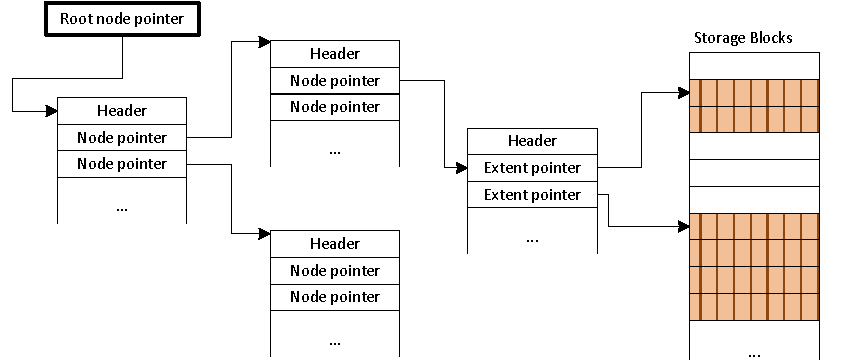
\includegraphics[width=0.7\textwidth]{figs/Ext4_extents.pdf}
        \label{fig:extent_tree}
      }
%      \hfill
      \subfloat[An extent/node pointer entry.]{
%      \centering
      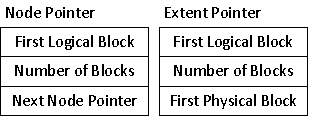
\includegraphics[width=0.3\textwidth]{figs/extent_feilds.pdf}
      \label{fig:extent_fields}
    }
%    \hfill

      \caption{The extent tree structure used for address translations.\label{fig:extent}}

\end{figure*}
%%%%%%%%%%%%%%%%%%%%%%%%%%%%%%%%%%%%%%%%%%%%%%%%%%

Figure~\ref{fig:extent_tree} illustrates the NeSC VF extent tree (which resembles the ext4 extent tree format). The extent tree is implemented as a B+ tree, each node contains only keys and the leaves contain the data itself.
A key is a tuple of (1) First Logical Block, which represents the first vLBA that the sub-tree beneath that key represents (2) Number of Blocks, which represents the amount of blocks the sub-tree represents. The data is an extent, which holds the translation from vLBA to pLBA. 
Each node in the tree comprises either a group of node pointers (the keys), which point to the next level of nodes, or a group of extent pointers, which are the tree leaves that point to the physical locations on the device. The header of each node indicates whether it contains node indices or extent pointers.

Figure~\ref{fig:extent_fields} illustrates the content of the entries in each type of node in the extent tree. Each \emph{extent pointer} entry consists of the first logical block it represents, a pointer to the first physical block of its extent, and the size of the extent. Each \emph{node pointer} entry comprises the first logical block it represents, the number of (non contiguous) logical blocks it covers, and a pointer to its array of child nodes.
%
If memory becomes tight, the hypervisor can prune parts of the extent tree and mark the pruned sections by storing NULL in their respective \emph{Next Node Pointer}. When NeSC needs to access a pruned subtree, it interrupts the host to regenerate the mappings.

Each  NeSC's VF is associated with an extent tree, which is stored in host memory, and the NeSC architecture (described in Chapter~\ref{chap:architecture}) stores the pointer to the root of each VF's extent tree. Whenever a VF is accessed, its extent tree is traversed using DMA accesses from the device to host memory. To mitigate the DMA latency, extents are cached on the NeSC device (more on this in Chapter~\ref{chap:architecture}).

Importantly, this use of software-defined, hardware-traversed per-VF extent trees eliminates the need to enforce protection and isolation in the hypervisor software layers, as discussed in Chapter~\ref{chap:motivation}. Instead, this task is offloaded to hardware and thereby mitigates one of the key performance bottlenecks of virtualized storage~\cite{le12nested}.

The per-VF extent tree model also enables the hypervisor to decouple the virtual device's size from its physical layout. This allows the hypervisor to initialize virtual devices whose logical size is larger than their allocated physical space, and to allocate further physical space when needed. This enables the hypervisor to maintain a compact physical representation of the stored data.

Finally, the NeSC design also enables multiple VFs to share an extent tree and thereby files. Nevertheless, NeSC only guarantees the consistency of the extent tree for shared files; it is up to the client VMs to address data synchronization and consistency issues.

\subsubsection{Root Filesystem}
\label{des:rootfs}
Through the PF, the hypervisor builds the root filesystem covering all the storage blocks of the device. With this filesystem the hypervisor manages the the allocation of blocks to VMs by using extent based files.
Every file on the filesystem represents a virtual disk, and the same mappings used by the filesystem to map file offsets to disk blocks, is used by NeSC to map vLBA accesses to pLBA on the device.
In modern filesystems, the extent tree is located on the storage device. Whenever the filesystem traverses the tree, it brings the node from the disk to memory and reads the LBA of the next block to bring. With NeSC,
the whole tree must always be in memory because the the device reads from it using DMA operations. Therefore the root filesystem keeps the tree pinned to physical memory and never on the device. 



%%%%%%%%%%%%%%%%%%%%%%%%%%%%%%%%%%%%%%%%%%%%%%%%%%%%%%%%%%%%%%%%%%%%%%
\section{Operational flow}
%%%%%%%%%%%%%%%%%%%%%%%%%%%%%%%%%%%%%%%%%%%%%%%%%%%%%%%%%%%%%%%%%%%%%%

%%%%%%%%%%%%%%%%%%%%%%%%%%%%%%%%%%%%%%%%%%%%%%%%%%
\subsubsection{Creating a new virtual disk}
%%%%%%%%%%%%%%%%%%%%%%%%%%%%%%%%%%%%%%%%%%%%%%%%%%
When creating a new virtual device, the hypervisor first creates the extent tree that will map the virtual device to physical blocks. Since the root  filesystems uses extent trees to map files to the physical layout, this stage typically consists of translating the root filesystem's own per-file extent tree to the NeSC tree format. The hypervisor will create a file on the root filesystem and the extent tree created will be used by NeSC for translating vLBA accesses for that virtual disk.
%
The hypervisor does not fully preallocate all the physical blocks needed for the new virtual device, this feature is called \emph{delayed allocation} in modern filesystems. When a new file representing a virtual disk is created, the
extent tree is empty and no physical blocks are allocated. Regardless of the size of the extent tree, the VF exposes the size of the virtual disk configured by the hypervisor. Blocks will be allocated only on demand, whenever a VM writes to
a block that isnt allocated, the hypervisor will allocate the block and update the tree.

The hypervisor then creates a new NeSC VF through the PF. It initializes the VF configuration registers (e.g., the size of the virtual device), writes the extent tree to  memory and sets the VF's base extent tree configuration register to point to the in-memory extent tree.

Following the two previous steps, the VF is ready and the virtual device is configured. The hypervisor then connects the VM to the new virtual machine, either by executing a new machine or by notifying an existing machine that a new device is available for its use (virtual device hotplug).
The new VF is mapped to a physical address and the hypervisor connects the virtual machine to the VF by mapping its \emph{guest physical address} to the physical address of the VF.
The guest OS will probe the PCIe bus and discover the VF.


%%%%%%%%%%%%%%%%%%%%
\begin{figure*}[!ht]

  \vspace*{-1.5ex}
  \centering
  \subfloat[Read Flow ]{
    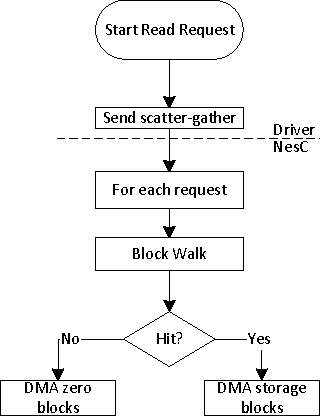
\includegraphics[width=0.4\columnwidth]{figs/read_flow.pdf}
 %   \caption{Read Flow}
    \label{fig:read_flow}
  }
  \hfill
  %% \vspace*{-1.5ex}
  \subfloat[Write Flow ]{
    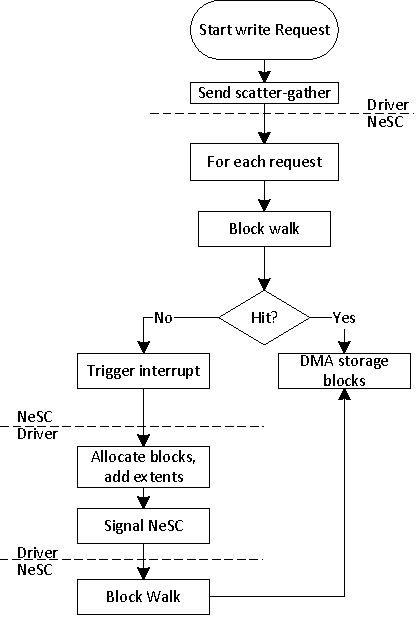
\includegraphics[width=0.5\columnwidth]{figs/write_flow.pdf}
%    \caption{Write Flow}
    \label{fig:write_flow}
  }
  \caption{Read and write flow in NeSC.\label{fig:flow}}
\end{figure*}
%%%%%%%%%%%%%%%%%%%%

%%%%%%%%%%%%%%%%%%%%%%%%%%%%%%%%%%%%%%%%%%%%%%%%%%
\subsubsection{Read flow}
%%%%%%%%%%%%%%%%%%%%%%%%%%%%%%%%%%%%%%%%%%%%%%%%%%
The read flow is depicted in Figure~\ref{fig:read_flow}. The VM's NeSC block driver is attached to the VF and can issue read requests to the device. Large requests are broken down by the driver to scatter-gather lists of smaller chunks. Our NeSC implementation operates at 1KB block granularity (which is, for example, the smallest block size supported by ext4), so the chunks sent by the block driver are broken down by NeSC to 1KB blocks. (more on this in Chapter~\ref{arch:drivers}) 
%
The device then translates each 1024 byte request address through the extent tree mappings of
that virtual function and creates a new queue of physical requests to read from physical storage
and DMA back to the host memory.

The translation of a vLBA to a pLBA can fail in one of two cases:
  1) The pLBA was never allocated due to lazy allocation. Following the POSIX standard, which dictates that unmapped areas inside a file (holes in the file) should read as zeros, NeSC transparently DMAs zeros to the destination buffer in host memory; or
  2) The pLBA was allocated, but its mapping was pruned from the extent tree due to memory pressure. NeSC identifies this case when it encounters a NULL node pointer when traversing the tree, and resolves it by sending an interrupt to the host and requesting that the hypervisor regenerates the pruned mappings (e.g., by re-reading the filesystem-specific mappings from disk).

%%%%%%%%%%%%%%%%%%%%%%%%%%%%%%%%%%%%%%%%%%%%%%%%%%
\subsubsection{Write flow}
\label{des:write}
%%%%%%%%%%%%%%%%%%%%%%%%%%%%%%%%%%%%%%%%%%%%%%%%%%

The write flow is shown in Figure~\ref{fig:write_flow}. Just like read requests, write requests are broken down by NeSC to 1KB chunks.

For each chunk, the device tries to perform vLBA-to-pLBA mapping using the VF's extent tree. If the translation succeeds, the data is written to the persistent physical storage.

Just like in the read case, the translation can fail due to unallocated blocks or pruned tree nodes. Both cases require NeSC to interrupt the hypervisor, which will request the filesystem for the mappings and rebuild the tree. The filesystem might have to allocate new blocks if this is the first time the vLBA is accessed. Once the hypervisor finishes handling the request, it signals NeSC to restart the extent tree lookup, which is now guaranteed to succeed.
%
If, however, the hypervisor cannot allocate more space for the VF (not shown in Figure~\ref{fig:write_flow}) due to a lack of physical storage or exhausted storage quotas, it signals an error to the PF which, in turn, triggers the VF to send a write failure interrupt to the requesting VM (we note that it is possible to optimize this process by delegating the interrupt directly to the VM~\cite{gordon12eli}).

%%%%%%%%%%%%%%%%%%%%%%%%%%%%%%%%%%%%%%%%%%%%%%%%%%%%%%%%%%%%%%%%%%%%%%
\section{Other design issues}
%%%%%%%%%%%%%%%%%%%%%%%%%%%%%%%%%%%%%%%%%%%%%%%%%%%%%%%%%%%%%%%%%%%%%%
\subsection*{Nested filesystems}
%%%%%%%%%%%%%%%%%%%%%%%%%%%%%%%%%%%%%%%%%%%%%%%%%%
A client VM will often manage its own filesystem inside its nested storage device. Given that a virtual device is stored as a file in the hypervisor's filesystem, this use case is commonly referred to as a nested filesystem.

Modern filesystems frequently use journaling for improved fault tolerance. This causes a well-known inefficiency in nested filesystems known as nested journaling~\cite{le12nested}. The inefficiency is caused as both the internal and external filesystems redundantly log the internal filesystem's data and meta-data updates. The common solution to this inefficiency is to tune the hypervisor's filesystem to only log meta-data changes for the file at hand and let the VM handle its internal filesystem's data integrity independently.

NeSC naturally lends itself to this common solution. Since NeSC VM clients directly access their data, the hypervisor's filesystem is not aware of the internal filesystem updates, whose integrity it handled by the VM, and only tracks its own meta-data updates.

%%%%%%%%%%%%%%%%%%%%%%%%%%%%%%%%%%%%%%%%%%%%%%%%%%
\subsection*{Direct storage accesses from accelerators}
%%%%%%%%%%%%%%%%%%%%%%%%%%%%%%%%%%%%%%%%%%%%%%%%%%

A straightforward extension of NeSC is to export data to accelerators in the system.
Traditionally, when an accelerator on the system wants to access storage, it must use the host OS as an intermediary and thereby waste CPU cycles and energy.

While not implemented in the prototype, we note that NeSC can be easily extended to enable direct accelerator-storage communications. This can be easily achieved by modifying the VF request-response interface, which is suitable for block devices, to a direct device-to-device DMA interface (in which offset 0 in the device matches offset 0 in the file, and so on.

This simple change to the VF interface enables accelerators to directly access storage using DMA, without interrupting the main processor and the OS. Such a design directly corresponds with the data-centric server concept presented by Ahn et al.~\cite{ahn2015dcs}

%%%%%%%%%%%%%%%%%%%%%%%%%%%%%%%%%%%%%%%%%%%%%%%%%%
\subsubsection*{Quality of Service (QoS)}
%%%%%%%%%%%%%%%%%%%%%%%%%%%%%%%%%%%%%%%%%%%%%%%%%%

Modern hypervisors support different QoS policies for each emulated disk image. Because the hypervisor mediates every disk access, it can easily enforce the QoS policy for each device. NeSC can be extended to enforce the hypervisor's QoS policy by modifying its DMA engine to support different priorities for each VF. Similar techniques are widely used by NICs that support SR-IOV.


%%%%%%%%%%%%%%%%%%%%%%%%%%%%%%%%%%%%%%%%%%%%%%%%%%
\subsubsection*{Unified buffer cache}
%%%%%%%%%%%%%%%%%%%%%%%%%%%%%%%%%%%%%%%%%%%%%%%%%%

  Different VMs often share storage blocks with one another.
  To minimize buffer duplication across VMs' buffer caches, common hypervisors use their own buffer cache as a unified buffer cache by forcing VMs to minimize their individual buffer caches (specifically, balloon drivers in each VM reclaim physical pages; the resulting memory pressure forces the VM to free buffered pages). As NeSC enables VMs to directly access storage, it prevents the hypervisor from maintaining a unified buffer cache. Instead, NeSC relies on memory deduplication to eliminate buffer duplication across guest VMs'. Notably, memory deduplication is supported by all modern hypervisors  (e.g., TPS in VMware, KSM in kvm and "Memory CoW" in Xen).  

